\documentclass[12pt, a4paper]{report}
\usepackage[utf8]{inputenc}
\usepackage[swedish]{babel}
\usepackage{relsize}
\usepackage[backend=biber, style=numeric-comp, sorting=none]{biblatex}
\usepackage{csquotes}
\usepackage{graphicx}
\usepackage{titlesec}
\usepackage{titling}
\usepackage{pgf-pie}
\usepackage[binary-units=true, abbreviations=true]{siunitx}
\usepackage{hyperref}
\usepackage{csquotes}
\usepackage{fancyhdr}
\usepackage{tocloft}
\pagestyle{fancy}
\lhead{Eddie Englund Gymnasiearbete TEINF17A VT 2020}
\rhead{\thepage}
\renewcommand{\headrulewidth}{0.4pt}
\renewcommand{\headheight}{14.999pt}

\setcounter{tocdepth}{3}
\setcounter{secnumdepth}{3}

\emergencystretch=1em

\setcounter{secnumdepth}{0}

\bibliography{bibliography.bib}
\addbibresource{bibliography.bib}

\author{Eddie Englund}
\title{Linux vs Windows\\[0.2em]\smaller{}En djupgående analys av prestandaskillnader mellan Microsoft Windows och Manjaro Linux}
\date{VT 2020}

\renewcommand{\abstract}{Abstract}
\renewcommand*{\bibfont}{\small}
\renewcommand*{\abstractname}{Abstract}

\makeatletter
\renewenvironment{abstract}{%
    \if@twocolumn
    \renewcommand*{\abstractname}{Abstract}

      \section*{\abstractname}%
    \else %% <- here I've removed \small
      \begin{flushleft}%
        \renewcommand*{\abstractname}{Abstract}

        {\bfseries \Large\abstractname\vspace{\z@}}%  %% <- here I've added \Large
      \end{flushleft}%
      \quotation
    \fi}
    {\if@twocolumn\else\endquotation\fi}
\makeatother


\begin{document}

\begin{titlepage}
    \maketitle

    \begin{center}
        \thispagestyle{empty}
    
        
\includegraphics[width=0.15\textwidth]{nti.png}\par\vspace{1cm}

    {\scshape\LARGE NTI Gymnasiet Gärdet \par}
    \vspace{1cm}
    {\scshape\Large Examensarbete, April 2020\par}
	\vspace{1.5cm}
    \textbf{
    Student: Eddie Englund, eddie.englund@elev.ga.ntig.se även eddie.englund@protonmail.com}
    \vspace{0.2cm}

    Handledare NTIG: Haris Kasumović, Haris.Kasumovic@ntig.se
    \vspace{0.1cm}

    Examinator NTIG: Haris Kasumović, Haris.Kasumovic@ntig.se
    
    \end{center}
\end{titlepage}

\setlength{\cftbeforetoctitleskip}{-3em}
\tableofcontents

\vspace{2cm}
\begin{abstract}
%% rewrite this
For every day that goes our world becomes more and more digitalised, and thanks to that we have lots and lots of options and there's lots of companies and startups that make everything from smart vacuum cleaners to smartwatches and cars. However, with options comes choosing one or more of them. In this analasys we will take a deep dive and look into the performance of two diffirent operatingsystems. Namely: Manjaro Linux and Windows 10. Because of this it's highly intresting to figure out if there's relevant performance diffirences between the two operating systems and to do so, low level languages/system languages will be used to make a benchmark to figure out if there's a relevant diffirence between Manjaro Linux and Windows 10.

\end{abstract}

\section{Sammanfattning}\label{sum}

I den här analysen så kommer det att tas reda på om Manjaro Linux och Windows 10 har olika prestanda och varför. Efter att att testen som skrevs hade körts så sa datan att Manjaro Linux var snabbare en Windows 10 med ungefär 10 mikro sekunder. Medans detta kan ses som mycket lite så måste vi komma ihåg att uppgiften som datorn utförde var att köra fibonacci sekvensen vilket är relativt lätt. Förvisso så är det så att prestanda testet bed fibonacci sekvensen kommer nära gränserna av 64bit så är det fortfarande relativt lätt. Så om det finns skillnader här (vilket det gör) så betyder det att om man skalar upp testerna på ett mycket större set så bör det teoretiskt sett var en högre prestanda skillnad. 
%% TODO: Finish this after you've finished the slutsats


\vspace{1cm}

    
\section{Inledning}
 
 
   I och med att världen blir mer och mer digitaliserad för varje dag som går, så är det inte konstigt att det finns en massiv marknad med olika alternativ för nästintill allting i den digitaliserade världen. Allt från telefoner till hemdatorer, robotdammsugare eller också en robotgräsklippare. Alla dessa digitaliserade mirakel har en sak gemensamt. Dem alla har ett operativsystem.
 
   Världens mest kända operativsystem\cite{winstat} är Microsoft Windows. Microsoft har en lång rad med olika versioner av sitt operativsystem\cite{windows}: Windows XP, Windows Vista, Windows 7[\dots] och deras senaste (och förmodligen sista) operativsystem Windows 10.
    
   Apple har flera olika operativsystem I deras olika produkter. I deras datorer så har dom macOS, i deras telefoner har dom iOS och i deras nya iPads så har dom iPadOS.\cite{appleOS}
    Det finns faktisk ett annat stort ``operativsystem''; Linux är en så kallad Kernel \cite{redhat} som är det man kan bygga ett operativsystem på. Linux har många olika operativsystem som är kallade för distributioner eller förkortat \textit{``distros''}. Linux är välkänt, speciellt inom utvecklar världen eftersom att det är mycket vänligt för utvecklingsmiljöer, dessutom så har Linux (oftast) en mycket god prestanda på maskiner med mindre processorkraft\cite{whatislinux}. På grund av detta så är bl.a: iPadOS, iOS, macOS, Android och nästintill allting annat som inte har så mycket processorkraft som t.ex en hiss någon form a Linux som operativsystem.

    Men vad är skillnaderna på dom här operativsystemen och är prestandan annorlunda mellan dom?
    
\section{Bakgrund/Teori}


    \subsection{Syfte/Frågeställning}
    Undersökningens syfte är att ta reda på om Linux eller Windows har olika prestanda och varför. Är det så att dom har olika prestanda i olika typer av applikationer eller är prestanda skillnaden konstant? Undersökningen kommer att använda en rad olika tester för att ta reda på om hypotesen nedan är sann.
 

    \subsection{Hypotes}

    Utifrån mina egen upplevelse så är Linux (när man väl har konfigurerat det ordentligt) en mycket mer stabil och snabbare upplevelse än Windows 10. I och med mina tidigare upplevelser så tror jag att Linux kommer att vinna. Linux kanske inte kommer att ha så mycket bättre resultat med stora marginaler men jag tror att Linux kommer att ha bättre prestanda.
    Det finns en anledning till att Linux finns i majoriteten av operativsystem men också i majoriteten av servers som cloud servers och liknande.
 

    \subsection{Linux}
 
   Linux är inte ett operativsystem. Däremot, så är Linux det som kallas för en ``kernel''\cite{redhat}. Det är hjärtat av operativsystemet eller kanske lite bättre jämfört med hjärnan av operativsystemet. Kerneln är en typ av mellanhand, mellan mjukvaran och hårdvaran. Den hanterar minnet, olika typer av processer, drivrutiner, systemanrop och säkerhet\cite{redhat}.
 

    \subsubsection{Distributioner}

   Eftersom att Linux är en kernel så finns det många så kallade distributioner/versioner (operativsystem). Skillnaderna mellan dem olika distributionerna kan variera högt, oftast handlar de största skillnaderna om vilka så kallad ``repositories'' (arkiv med mjukvara) man använder för att distribuera mjukvara. Dessutom så kan det handla om vilka filsystem man använder men också hur mycket eller hur lite förinstallerade program som finns när man installerar distributionen.

   \subsubsection{Repositories}

    En högt definierande egenskap hos Linux är användandet av ``repositories''. Repositories är arkiv eller en databank med mjukvara. Man använder sig utav dessa för att lättare och säkert installera program.

    Normalt sett när man ska installera ett program på Windows eller Mac så öppnar man en webbläsare och söker på mjukvaran man vill ha, går till sidan, laddar ner en program installatör för det programet man vill ha, sedan kör man den. Efter det kan man ta bort installatören(om man kommer ihåg att göra det).
    
    Men inte på Linux. På Linux så använder man oftast sig av en terminal och ett kommando (detta varierar på distron).
    På Manjaro som är Arch baserad så använder man sig utav pacman\cite{pacman}. Pacman är en ``package manager''\cite{pkgmanager}. Den hanterar paket (mjukvara) som man vill ta bort, installera eller kanske uppdatera.

    För att installera ett program på Manjaro så skulle man skriva: sudo pacman -S programnamn. Notera att det går att installera program på andra sätt


    \subsubsection{Absolut kontroll}

   En annan fördel med Linux är att man har absolut kontroll. Man kan byta så kallade \textit{window managers} eller förkortat \textit{wm}\cite{wm}. Man kan även göra om Linux kerneln ifall man vill göra något specifikt eller kanske inte behöver bitar av den för att optimera sin maskin. Detta är mycket vanligt inom låg processor kraftiga maskiner som hissar eller smartklockor.

   Allt detta är tack vare att Linux har en öppen källkod och tillåter användare att göra vad dom vill med det. Detta skulle aldrig vara möjligt på Windows eller Mac (om man inte crackar/gör illegala saker) eftersom att deras licenser säger att man inte får och dessutom så får man inte distribuera sina ändringar ifall man har gjort dem.

   \subsubsection{Öppen källkod}


   Den största skillnaden mellan Linux och Windows är att Linux inte är proprietär och har öppen källkod vilket betyder att vem som helst kan bidra med kod för att göra kerneln eller distributionen bättre och dessutom lägga till fler användbara funktioner, men även också att fixa buggar. Öppen källkod har även en annan fördel och det är att koden oftast inte är så kallad \textit{``bloated''}, alltså att det finns kod eller funktioner som inte behövs eller att kod kvaliteten inte är bra. Detta leder till att prestandan på Linux är mycket hög.

   \subsection{Windows}


    \subsubsection{Skrivet I flera språk}
    
    Windows 10 är skrivet i programeringsspråket C\# som är skapat av Microsoft\cite{c}. Microsoft skapade C\# för 20 år sedan (2000) när de ville skriva delar av Windows XP i Java men det fick dem inte eftersom att Oracle sa nej. Så de utvecklade vad Klaus och Angelika Langer sa i ett bloginlägg att ``Java and C\# are almost identical programing languages. Boring repetition that lacks innovation''.\cite{cquote}  
    

    \subsubsection{Proprietärt}
    Windows är också ett operativsystem som är skrivet helt ``in house'' (det är inte öppen källkod).
    Eftersom att det inte är öppen källkod så vet vi inte riktigt va Windows faktiskt håller på med i bakgrunden. Det gör så att man inte kan ändra på saker lika mycket som man kan på Linux. Dessutom så gör det att Microsoft kan göra lite vad det vill eftersom att det inte måste informera sina användare om alla ändringar (om inte lagen kräver det). Dessutom så är Windows ganska restriktivt i och med att man inte har absolut kontroll över bl.a när man ska/vill uppdatera.


   Men det finns faktiskt en fördel med att inte ha öppen källkod. Microsoft kan skapa en virtuell monopoli över vissa marknader. T.ex så är Windows (inom pc världen) det bästa operativsystemet att spela på. Det här är eftersom att dom flesta spelen är skapade för att köra på Windows. Det är eftersom att DirectX\cite{directx} finns på Windows men också eftersom att det inte är öppen källkod så är det inte särskilt lätt att piratkopiera spelen och deras innehåll.


 
\section{Metod}
 
\subsection{Distribution}
Den distributionen som jag har valt att använda är Manjaro\cite{manjaro}. Manjaro är en så kallad \textit{Arch based distro}. Den är baserad på en annan distro som heter Arch Linux som ofta blir kallat för en av dom bästa distributionerna\cite{archIsTheBest}. Däremot så gör Manjaro det lättare att komma igång och så har Manjaro dem flesta fördelarna som Arch Linux har.

\subsection{Språk och program}
 
För att ta reda på om det finns prestandaskillnader mellan Windows och Linux (manjaro) så behövde jag ta reda på vilket programeringsspråk som vore relevant för att mäta prestandan mellan Windows och Linux(Manjaro) och en del andra saker.

\begin{enumerate}
   \item Vilket programeringsspråk bör användas och varför?
   \item Vad bör man utföra för uppgift i programet för att få maskinerna att arbeta?
   \item Hur mäter vi prestandan?
   \item Hur kan vi verifiera våra mätningar?
\end{enumerate}
 

\subsubsection{Val av programeringsspråk}

När jag skulle ta reda på vilket programeringsspråk jag skulle använda för att skriva benchmarket, spenderade jag mycket tid till att läsa litteratur kring programeringsspråk. Detta var mycket svårt eftersom att det finns extremt många programeringsspråk. Bara för att nämna ett par: Java, Javascript, Python, C, C++, C\#, Ruby, Rust, mm. 


Efter att jag hade läst litteraturen relaterande till programeringsspråken så kom jag fram till att jag skulle skriva mitt program i språket Rust.\cite{rust} Anledningen till detta är att Rust är ett snabbt, stabilt och ett ``systemnivå språk''. Dessutom så har Rust lite så kallat \textit{``garbage collection''}\cite{garbage}, alltså att Rust bl.a gör sig av med oanvända variabler som tar platts i RAM-minnet. Dessutom så valde jag Rust över C och C++ eftersom att jag har använt mig av det tidigare.

Jag valde att ta bort programeringsspråken som var långsamma och de programeringsspråk som är \textit{``interpreted''}\cite{Interpreted-language}. Dessutom så tog jag bort språken som har kompabilitets lager. Dessa kritierer tog bort: Java, Javascript, Ruby, C\# och Python.

\subsubsection{Vad ska programmet utför för uppgift, hur mäter jag prestandan och hur verifierar jag mina resultat?}

Ett problem som uppstod när jag först försökte fylla en vektor med 1 gigabyte utav integers och sedan loopa programet för att ha det igång så att jag kan verifiera att den gör det den ska, så la jag snabbt märke till att programet inte tog i närheten så mycket som jag hade sagt åt språket att göra.

Så jag gjorde en del research och det visar sig att Rust till skillnad från C och C++ har lite så kallad ``garbage collection'' som är mycket smart. Om datan inte blir använd så är den datan inte registrerad utan data platsen i ram minnet är endast reserverat. Så jag fick ta ett steg tillbaka och tänka på vad jag kan göra istället.
 
Jag kom senare på en idé om att använda mig av ett bibliotek som heter ``criterion'' som är användbart för att göra så kallade ``benchmarks'', alltså att mäta prestandan. Med det biblioteket så skrev jag ett kort program som kör fibonacci sekvensen och kalkylerar den. Det är en mycket tung process som börjar trycka på gränserna av 64bit. Efter det så kör jag prestanda testet 20 gånger och sedan så tar jag genomsnittet av alla test värdena för att se till att testerna är precisa och exakta.
 
 
\subsection{Vad tror utvecklare?}
 
   För att ta reda på vad andra utvecklare har för hypotes/teori om prestandan mellan Linux och Windows 10, varför prestandan skulle vara annorlunda, vilket operativsystem de föredrar och varför, så delades det runt ett formulär runt omkring olika programmerings/utvecklingsforum men även genom kontakter lyckats skicka vidare enkäten i professionella utvecklingsmiljöer.
 
   Notera att enkäten var skrivet på engelska för att kunna nå ut till så många utvecklare så möjligt.
    
   \vspace{1cm}
 
 
   \small{OBS! Det fanns några frågor som var alternativa, till exempel: att motivera sina svar.
  
   Vill ni läsa dessa motiveringar så finns dom här:} \smaller{\url{https://tinyurl.com/rccw2af}}
 
\vspace{1cm}
\section{Resultat}

    \subsection{Enkät}   \label{form}

\large {Which operating system would have superior performance in tasks like, compiling code, executing code or even intensive workloads like working in a program  like blender or unity?}
 
   \vspace{.5cm}
 
   \normalsize I denna fråga så frågades olika utvecklare vad de trodde kring Linux. Tror dom att Linux eller Windows har bättre prestanda när det kommer till att kompilera/köra/använda olika applikationer/program?
 
 
   \vspace{1cm}
 
   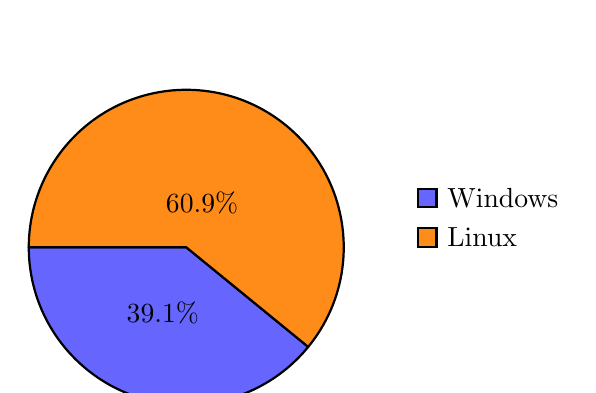
\begin{tikzpicture}
       \pie [rotate = 180, color = {blue!60, orange!90}, radius = 2, text = legend]
   {39.1/Windows,
    60.9/Linux}
 
   \end{tikzpicture}
 
   \cite{form}


   I denna fråga så tog man reda på att 60.0\% av 23 svar, ansåg att Linux skulle ha högre prestanda en Windows.

    \vspace{.5cm}
    I enkäten så läts deltagarna motivera sina tankar (inte obligatoriskt). Ett mycket välmotiverat svar: \begin{displayquote}I don't have much, just wanted to say that linux will ofc perform better in day to day tasks due to the fact that it consumes less resources in the first place

    on another note, let the numbers speak by themselves \hyperlink{https://www.phoronix.com/scan.php?page=article&item=win10-debian101-intel} [\dots] just in general, the flexibility that linux provides is the main reason it performs better, as you can fit it much better to the job to have the maximum performance of your hardware

    the way you compile the kernel can drastically change the performance of linux over an application, this can depend on the architecture and instructions you use to compile, small tweaks like buffer sizes to allow for better scalability on very high core count cpu's, the compiler you use like ICC for intel, AOCC for Amd, Clang, GCC, etc..\end{displayquote}

Det här svaret från en av applikanterna är lik och en del av min egen hypotes (läs mer om detta på sida: \pageref{slutsats})


   \vspace{3cm}
 
   \large{If you had the option to choose between Windows and Linux which one would you choose? (of course, you can choose any distro for Linux)}
  
   \vspace{.5cm}
  
   \normalsize I Denna fråga så frågar vi utvecklare vilket operativsystem de skulle välja om de hade chansen. Vi fick ett ganska fascinerande resultat. Om vi hade fått ett jämt antal svar så hade det varit en rak 50 50 på denna fråga men den tjugotredje personen som svarade på frågan valde Linux över Windows.
 
   \vspace{1cm}
 
   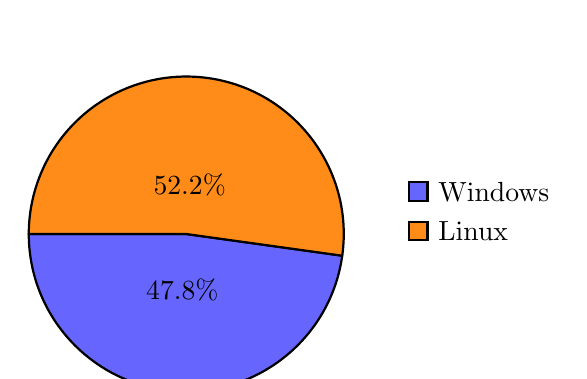
\begin{tikzpicture}
       \pie [rotate = 180, color = {blue!60, orange!90}, radius = 2, text=legend]
   {47.8/Windows,
    52.2/Linux}
 
   \end{tikzpicture}
 
   \cite{form}
 
   \vspace{1cm}

   \subsection{Prestanda skillnader}\label{tests}

   \subsubsection{Linux(Manjaro)}
   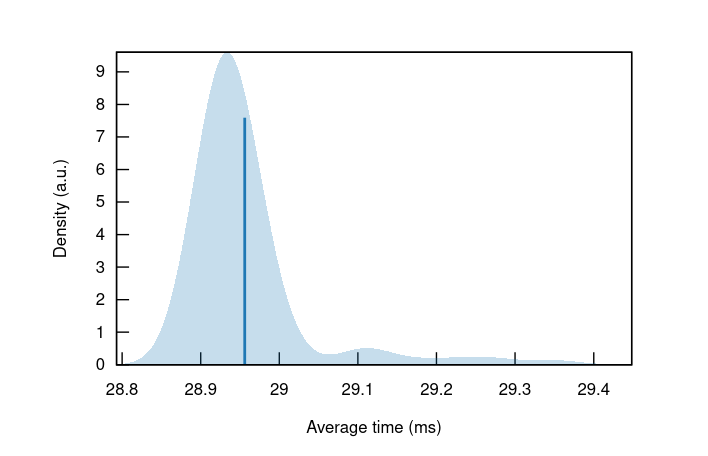
\includegraphics[width=1\textwidth]{bench_linux_average_time}
   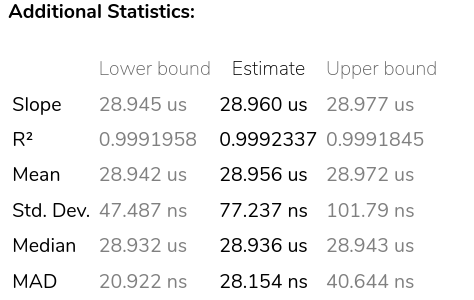
\includegraphics[width=.8\textwidth]{add_stats_linux}

   Notera att en fel gjordes när graferna var skapade. Det ska \textbf{INTE} stå ``Average time (\textbf{ms})'' utan det ska stå ``Average time (\textbf{us}) alltså mikrosekunder.
   \subsection{Windows 10}
   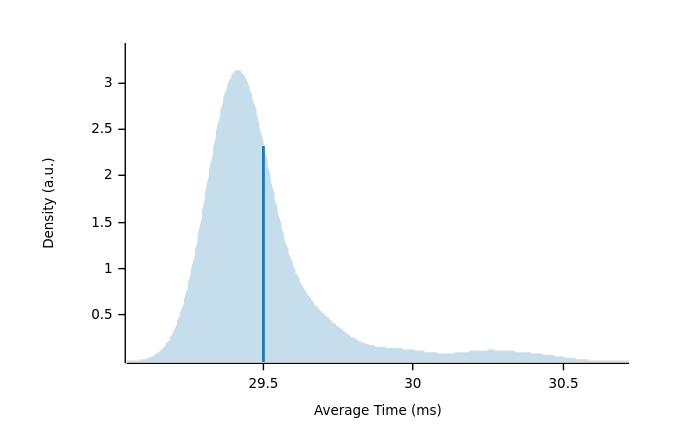
\includegraphics[width=1\textwidth]{bench_windows_average_time}
   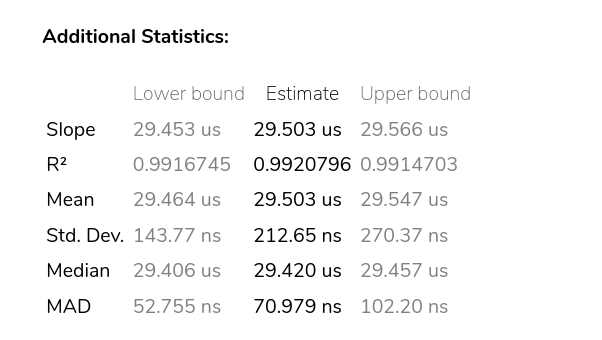
\includegraphics[width=1\textwidth]{add_stats_windows}

   Notera att en fel gjordes när graferna var skapade. Det ska \textbf{INTE} stå ``Average time (\textbf{ms})'' utan det ska stå ``Average time (\textbf{us}) alltså mikrosekunder.

\section{Analys/diskussion}

\subsection{Enkät}

\subsubsection{Fråga 1}
Den första frågan var inom förväntningar. Anledningen till detta är att alla utvecklare inte känner till Linux på en djupare nivå än att Ubuntu är en av dom vanligasta distributionerna\cite{commondistro}.

\subsubsection{Fråga 2}
Den andra frågan var däremot ganska förvånande i och med att 52.5\% av som svarade skulle välja Linux över Windows om de hade chansen. Detta är ganska förbryllande eftersom att Linux är välkänt för att kräva mycket konfiguration och/eller datorintresse. Man kan tänka sig att många utvecklare skulle vara högt dator intresserade men det är inte sant (enligt min upplevelse i och kring forum). Många frontend utvecklare använder sig ofta av proprietära program som Adobe Experience Design (Adobe Xd). 


\subsection{Benchmark}

Enligt test resultaten (se sida:\pageref{tests}) så kan man se att Manjaro Linux har bättre prestanda en Windows 10 med ungefär 10 mikrosekunder. Medans detta kanske inte ser ut som speciellt mycket skillnad så är det mycket möjligt add dena mikro skillnad blir mycket större när man använder sig utav fler tunga programm/processer sammtidigt.

Detta kan man se och förstå när man tittar på användningen av Linux i servers.

\vspace{1cm}
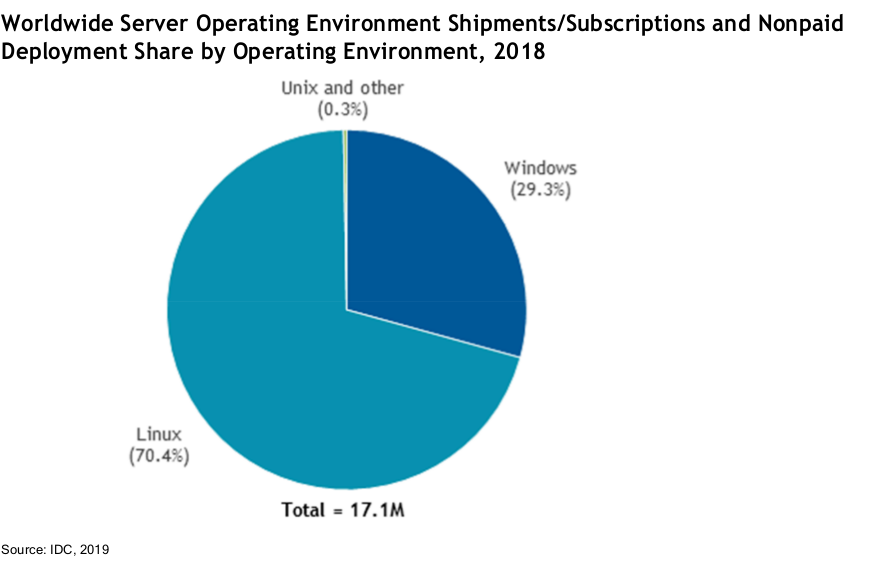
\includegraphics[width=.6\textwidth]{IDC.png}\cite{linux-market}


\subsection{Problem med metodiken}

\subsubsection{Enkäten och vinklad data}

Vinklad data kan och är förmodligen ett problem med enkäten som jag har skickat ut. Anledningen bakom den vinklade datan som jag har fått ut av enkäten är ställena jag har skickat ut det. Jag har skickat enkäten på design/web/programmerings relaterade forum och även skickade det via min mor som är team leader för en grupp utvecklare. Om jag hade skickat enkäten på andra mer publika medium så hade förmodligen datan sett mycket annorlunda ut eftersom att majoriteten av befolkning inte känner till Linux även dock det finns över allt runt om kring oss (dem finns i våra telefoner, datorer, klockor, mm.). 

\subsection{Okända variabler som skulle kunna ha effekt på resultatet}


\subsubsection{Använd Mjukvara}

Om man ska utföra ett så precist benchmark så möjligt när det kommer till mjukvara så bör man ha helt nya verisioner och inga andra program som inte är nödvändiga. Detta eftersom att annars kan det finns oidentiferade program eller bakrundsproccesser som tar upp prestanda. Detta kan leda till att det finns fler bakrundsproccesser igång vilket teoretiskt sett skulle kunna leda till försämrade resultalt.

Om jag skulle kunna gjort det, så skulle jag ha rensat min maskin helt och ominstallerat båda operativsystemen och sedan endast installerat de paket/mjukvara jag behöver.

\subsubsection{Datorer och värme}

Alla datorer kräver elektricitet. Min CPU (Amd ryzen r7 1700 \SI{3.0}{\giga\hertz}) drar \SI{65}{\watt}(TDP)\cite{ryzen1700spec} men den kräver förmodligen mer en så eftersom att jag har överklockat min CPU till \SI{3.9}{\giga\hertz}.
Dessutom så har jag en GTX 1070 Armored OC från MSI\cite{1070} och den drar \SI{150}{\watt}.

Eftersom att det finns el i systemet så kräver det att man kyler ner det på grund av spillvärme\cite{wasteheat} som man måste bli av med för att kunna behålla prestandan. Kylningen är nästan aldrig konstant om man inte har en värme kontrollerat rum eller låda. Eftersom att jag inte har det så kan jag inte garantera mina resultat eftersom att jag gjorde dom på olika dagar och vid olika tidpunkter. Detta gör att rumstemperaturen kan vara annorlunda. En dator kan aldrig bli kallare än vad rummet är\cite{thermodynamics} om man inte använder sig av kemikalier som Ln2.



\section{Slutsats}\label{slutsats}

Analysen har gått mycket bra och analysen visar att Manjaro Linux har högre prestanda en vad Windows 10 har (se sida: \pageref{tests}). Jag anser dock att för att definitivt säga att Linux har högre prestnada en Windows så bör det testas på fler sett en vad jag har kunnat göra i denna analys. Några ideer gällande vad man bör testa vore: grafik relaterade processer som Blender\cite{blender} och/även standardiserade tester som t.ex Indigo Bench\cite{indigo}. Detta eftersom att det finns olika typer av prestanda att mäta. Bara för att nämna ett par: fps (frames per second), kompilerings tider, exekveringstider, mm.


\printbibliography[type=online]

\printbibliography[type=misc, title={Bilagor}]


\end{document}


%% Note to self:

%% Write about how Linux stays ahead in security and performance by switching to newer versions of File systems and other systems/software.
